\section{Dynamic World Model Construction}\label{sec:construction_pipeline}
Dynamic world model construction refers to the end-to-end process by which raw sensor observations are transformed into a persistent, probabilistically grounded, and semantically structured representation of a non-stationary environment. 
In hybrid representations combining factor graphs and scene graphs, this process spans multiple tightly interacting stages, from front-end perception and data association to back-end inference and long-term graph maintenance.

Rather than a monolithic pipeline, modern systems adopt modular yet interdependent components, where design choices at early stages (e.g., detection granularity or association strategy) strongly influence the stability, scalability, and expressiveness of the resulting world model under dynamics.
This section organizes existing approaches around four core stages that recur across the literature: front-end perception (Section \ref{sec:construction_pipeline_frontend}), data association (Section \ref{sec:construction_pipeline_data_association}), back-end inference and optimization (Section \ref{sec:construction_pipeline_backend}), and graph maintenance (Section \ref{sec:construction_pipeline_graph_maintenance}).
A general pipeline overview is depicted in Figure \ref{fig:FG_SG_world_model_construction_maintenance_workflow}.

\subsection{Front-End Perception}\label{sec:construction_pipeline_frontend}
The front-end perception stage is responsible for extracting candidate entities, attributes and relations from raw sensor data.
In dynamic environments, this stage must operate under partial observability, occlusion and motion ambiguity, while providing sufficiently rich primitives for downstream probabilistic inference. 

\subsubsection{Geometric and Semantic Primitives}
At the geometric level, front-ends extract low-level features such as points, lines, planes or surfels, which remain the backbone of factor graph-based SLAM systems \cite{dellaert_factor_2017} \cite{rosinol_kimera_2021}. 
However, dynamic scenes increasingly require object- and agent-level primitives, motivating the integration of instance segmentation, 3D bounding volumes, or parametric object models \cite{bescos_dynaslam_2021} \cite{morris_dynosam_2025} \cite{schmid_khronos_2024}.

Semantic perception pipelines typically produce:
\begin{itemize}
    \item \textbf{Object detections and instances}, often class-labeled and possibly open-vocabulary \cite{yan_dynamic_2025} \cite{gu_conceptgraphs_2023};
    \item \textbf{Agent hypotheses}, including humans or vehicles, sometimes with articulated or rigid-body structure \cite{henning_bodyslam_2022} \cite{qiu2022airdos};
    \item \textbf{Attribute estimates}, such as object state (open/close, on/off) \cite{olivastri_multi-modal_2024};
    \item \textbf{Relation hypotheses}, e.g., spatial (on, in, next-to) or functional (controls, supports) \cite{catalano_3d_2025} \cite{zhang_open-vocabulary_2025}.
\end{itemize}

In hybrid FG-SG systems like Kimera \cite{rosinol_kimera_2021} or Khronos \cite{schmid_khronos_2024}, these outputs are deliberately redundant: dense geometric observations coexist with higher-level semantic abstraction, resulting in robustness to perception failures. 

\subsubsection{Temporal Grouping and Tracking}
To cope with dynamics, front-ends often incorporate \textit{short-term temporal aggregation}, producing tracklets or object fragments prior to global optimization. 
Optical flow, frame-to-frame association, or local tracking modules are commonly used to stabilize detections before they enter the global world model \cite{morris_dynosam_2025} \cite{schmid_khronos_2024}.
Khronos \cite{schmid_khronos_2024}, for example, explicitly constructs temporally consistent object fragments ahead of the active-window integration described in Section \ref{sec:dyn_world_model_representations_scene_graphs}, postponing commitment to the global model until sufficient evidence is accumulated.

This early temporal coherence reduces spurious node creation and limits the combinatorial computational effort on later data association stages.
From an end-to-end perspective, these front-end mechanisms constitute the first error-containment stage of the world-model pipeline: temporal aggregation can suppress isolated false detections or noisy estimates before they become persistent graph entities.
Conversely, systematic missed detections or misclassifications that survive this stage are passed to association and graph construction, where they may become persistent structural errors.

\subsection{Data Association}\label{sec:construction_pipeline_data_association}
Data association is the process of determining which observations correspond to which existing entities in the world model, or whether they should instantiate new ones. 
In dynamic environments, association errors are among the primary failure reasons, as incorrect correspondences can propagate across time,  corrupting both geometric estimation and semantic structure. 

\subsubsection{Deterministic and Probabilistic Association}
Classical SLAM systems rely on deterministic association mechanisms, such as nearest-neighbor matching or Hungarian assignment based on geometric or appearance similarity \cite{lingzhu_xiang_robust_2015} \cite{gou_visual_2024}. 
While efficient, these approaches degrade quickly under occlusion and fast motion.

To address this, many dynamic-world-model systems employ \textit{probabilistic multi-hypothesis association}, including:
\begin{itemize}
    \item \textbf{Joint Probabilistic Data Association (JPDA)}, which marginalizes over multiple correspondence hypotheses \cite{gulati_robust_2017};
    \item \textbf{Multiple Hypothesis Tracking (MHT)}, which explicitly maintains competing association trees over time \cite{zaech_learnable_2022};
    \item \textbf{Learned association}, where neural embeddings (e.g. CLIP features) define similarity metrics for object re-identification \cite{gu_conceptgraphs_2023} \cite{yan_dynamic_2025}.
\end{itemize}
In factor-graph formulations, association decisions are often represented implicitly via latent correspondence variables or explicitly through switchable or weighted constraints \cite{giberna_dynemo-slam_2025} \cite{lingzhu_xiang_robust_2015}.
This association uncertainty is distinct from geometric-state uncertainty. A small pose covariance conditioned on an incorrect correspondence does not imply that the correspondence itself is reliable, motivating explicit treatment of competing association hypotheses.

Data association is therefore a particularly critical propagation interface.
Unlike continuous measurement noise, which often can be reduced by additional observations, committing an observation to the wrong entity changes which states are connected by subsequent factors and may contaminate both the estimated geometry and the semantic history of that entity.

\subsubsection{Association under Dynamics}
Dynamic environments need distinguishing between moving agents, movable but stationary objects, and ephemeral observations, like transient clutter or false positives.
Several works incorporate \textit{movability or existence variables} to mediate association decisions \cite{brink_using_2016} \cite{gomez_object-based_2020}.  
From a probabilistic perspective, Random Finite Set (RFS)-based formulations (Section \ref{sec:construction_pipeline_graph_maintenance}) provide a mechanism for handling association, birth and death jointly \cite{ristic2013tutorial} \cite{garcia2018poisson}, although full integration with scene graph construction remains limited.
Open-vocabulary embeddings extend data association beyond predefined semantic classes, but they primarily provide semantic generality rather than a probabilistic association model. 
Their similarity scores should therefore not be interpreted as equivalent to posterior association probabilities produced by multi-hypothesis methods such as JPDA or MHT. This distinction becomes particularly important under dynamics, where visually similar objects, occlusion, and viewpoint change can produce confident but incorrect semantic matches.

\subsection{Back-End Inference/Optimization}\label{sec:construction_pipeline_backend}
The back-end integrates associated observations into a globally consistent world model, resolving the geometric, semantic and temporal constraints through probabilistic inference.

\subsubsection{Incremental Factor Graph Optimization}
Most modern systems rely on \textit{incremental smoothing} over factor graphs, using solvers such as iSAM2 \cite{kaess2011isam2} or g2o \cite{kummerle_g2o_2011} to maintain real-time performance under continuous updates \cite{dellaert_factor_2017} \cite{morris_dynosam_2025} \cite{bavle_situational_2022}.
Variables typically include robot poses, static landmarks, dynamic object states, and sometimes higher-level structural entities (walls, rooms) \cite{bavle_s-graphs_2025}.

Dynamic environments additionally introduce new challenges:
\begin{itemize}
    \item \textbf{Spatio-temporal factors} couple robot motion and object motion \cite{morris_dynosam_2025} \cite{zhang_semantic-integrated_2026};
    \item \textbf{Switchable or robust factors} downweight inconsistent measurements caused by dynamic entities \cite{song_rts-slam_2025} \cite{lingzhu_xiang_robust_2015};
    \item \textbf{Motion priors} (e.g. constant velocity) regularize underconstrained trajectories \cite{morris_dynosam_2025} \cite{giberna_dynemo-slam_2025} \cite{bescos_dynaslam_2021}.
\end{itemize}

\subsubsection{Continuous Motion Modeling}
Continuous dynamics are primarily modeled as trajectories of robot poses ($\mathit{X}_k$) or dynamic object poses ($\mathit{L}_k$) and motions ($\mathit{H}_k$).
% world-centric object-centric (hybrid) formulations
Morris et al. \cite{morris_importance_2024} highlight a fundamental dichotomy in coordinate frame representation, presenting World-Centric and Object-Centric Formulations.
Traditional object-centric models express dynamic points in a local body frame, where they appear static.
However, this necessitates estimating the pose of each object at every timestep, often leading to instability because these frames are not directly observable. 
On the other side, world-centric representations describe rigid-body motion directly using variables in the world frame. 
Recent ``hybrid'' formulations \cite{morris_online_2025} anchor motion to an embedded frame ($\mathit{L}_e$) initialized upon the first observation, which preserves factor graph sparsity and enhances convergence for incremental solvers like iSAM2. 

% kinematic motion models
When it comes to the design of kinematic motion models, most frameworks adopt a constant velocity model\cite{bescos_dynaslam_2021} \cite{morris_dynosam_2025}, to regularize the optimization problem. 
Some higher-fidelity models include constant acceleration \cite{brink_using_2016} or specific zero velocity priors to handle humans or robots that may remain stationary for intervals of time \cite{rosinol_3d_2020}.
Such motion models are themselves uncertain priors rather than deterministic constraints: their associated covariance controls how strongly deviations from the assumed dynamics are penalized. Underestimating this model uncertainty can over-constrain trajectories when an entity violates the assumed motion pattern, whereas overestimating it reduces the regularizing benefit of the prior.

%spatio-temporal factors
These motion priors are realized in the back-end through spatio-temporal factors that couple camera poses with object motion vertices, introducing cross-terms in the Hessian matrix that improve accuracy and efficiency compared to independent spatial factors \cite{zhang_semantic-integrated_2026}.

\subsubsection{Loop Closure and Multi-layer Consistency}
Loop closure remains essential for long-term consistency but is particularly risky under dynamics. 
Incorrect loop closures induced by moved objects or agents can catastrophically corrupt the map \cite{giberna_dynemo-slam_2025}.
Systems like Khronos \cite{schmid_khronos_2024} and DPG-SLAM \cite{walcott-bryant_dynamic_2012} delay or gate loop closure decisions using geometric verification and temporal consistency checks.

In hybrid FG-SG systems, back-end inference must also ensure \textit{cross-layer consistency}. 
First, geometric optimization updates metric nodes poses. 
Furthermore, scene graph abstractions (e.g. room belonging and containment relations) must be updated accordingly. 
Unified optimizable representations, like S-Graphs \cite{bavle_s-graphs_2025}, handle this naturally, while layered architectures require explicit synchronization policies \cite{hughes_hydra_2022} \cite{rosinol_kimera_2021}.

\subsection{Graph Maintenance}\label{sec:construction_pipeline_graph_maintenance}
Beyond inference, dynamic world models must remain computationally tractable, stable and meaningful over long time horizons. 
Graph maintenance governs how nodes and edges are added, updated, kept, or removed.

\subsubsection{Node Lifecycle: Birth, Persistence, Death}
Entity lifecycle management is central in dynamic environments. 
Common strategies include:
\begin{itemize}
    \item \textbf{Evidence accumulation thresholds} for node birth \cite{schmid_khronos_2024};
    \item \textbf{Temporal decay or confidence scores} governing persistence \cite{gomez_object-based_2020};
    \item \textbf{Geometric verification} (e.g. ray tracing) to distinguish occlusion from true removal \cite{schmid_khronos_2024}.
\end{itemize}
%Probabilistic treatments model existence explicitly, as in Bernoulli or PMBM filters \cite{ristic2013tutorial} \cite{garcia2018poisson}, offering a principled alternative to heuristic approaches.

These heuristics can be grounded in a more principled probabilistic treatment.
The Random Finite Set (RFS) framework elevates birth and death from heuristic thresholds to first-class elements of the Bayesian filtering recursion \cite{ristic2013tutorial}. 
In this formulation, the set of tracked entities is itself a random variable, and existence is modeled explicitly through a binary latent variable $\epsilon_k \in \{0,1\}$ evolving as a first-order Markov chain with transition probabilities $p_B$ (birth) and $p_S$ (survival). 
The Bernoulli filter propagates an existence probability $r_k \in [0,1]$ alongside the spatial density, decomposing additively into a survival term $p_S \cdot r_{k-1}$ and a birth term $(1-r_{k-1})\cdot p_B$ \cite{ristic2013tutorial}. 
This formulation has a direct and underexplored connection to dynamic world models: each scene graph node representing a potentially transient entity, e.g. a movable chair, a walking human, a momentarily occluded object, can in principle be equipped with such an existence probability, making node lifecycle a Bayesian inference problem rather than a threshold-based engineering decision.
Existence uncertainty should therefore be distinguished from both state-estimation and data-association uncertainty. Conditioned on an entity existing and being correctly associated, its pose may be accurately estimated, while the probability that the entity still exists can nevertheless remain low or uncertain.

The Probability Hypothesis Density (PHD) filter extends this to the multi-entity case by propagating the first-order moment of the multi-target posterior, avoiding explicit data association while jointly estimating the number and locations of dynamic entities \cite{mullane2011random}. 
Its application to SLAM \cite{mullane2011random} showed that modeling the landmark map as an RFS rather than a random vector provides a principled treatment of feature appearance, disappearance, missed detections and clutter within a single Bayesian recursion, and has since been applied directly to SLAMMOT \cite{siew2018simultaneous}. 
This separation into a static factor graph layer and a dynamic PHD layer mirrors the architectural splits between the factor graph backbone and the dynamic node layer of hybrid FG-SG systems.

For the full multi-entity case with explicit track management, the Poisson Multi-Bernoulli Mixture (PMBM) filter provides a Bayes-optimal conjugate prior \cite{garcia2018poisson}. 
A Poisson Point Process describes the existence of yet undetected targets, while a Multi-Bernoulli Mixture describes the distribution of already-detected targets \cite{granstrom2019poisson}. 
This maps naturally onto robotic world modeling: undetected entities correspond to the PPP intensity, while confirmed tracks carry an explicit existence probability $r_k^i$ updated at each timestep \cite{deusch2015labeled}, with track pruning by thresholding \cite{reuter2014labeled}. 
The PMBM formulation has been extended directly to SLAM \cite{kim2022pmbm}, and more recently combined with a graph-based SLAM back-end \cite{ge2025batch} to bridge RFS-based entity management with factor graph optimization.

The appearance rate of new entities can itself be modeled with a Poisson process of intensity $\lambda_B(\cdot)$ over the state space \cite{garcia2018poisson}; non-homogeneous variants let this birth intensity adapt over time, capturing phenomena such as increased agent density during peak hours \cite{li2023adaptive}. 
This connects naturally to Aion's MoD (Section \ref{sec:dyn_world_model_representations_scene_graphs}), readable as a time-varying birth intensity learned empirically over navigational nodes rather than specified a priori. 
Semantic extensions such as the Semantic PHD filter \cite{chen2019multi} further augment existence estimation with class labels, bridging the RFS tracking layer and the semantic node types of scene graphs.

Ray-tracing offers a geometric instantiation of this Bayesian update: if a ray from the robot's current pose to a background vertex passes through a previously mapped object's volume and returns a longer-than-expected depth, the system confirms removal rather than occlusion \cite{schmid_khronos_2024}. 
Belief Scene Graphs' blind nodes (Section \ref{sec:dyn_world_model_representations_scene_graphs}) correspond conceptually to the PPP component of the PMBM framework, a distribution over undetected but plausible entities, though implemented via Graph Convolutional Networks rather than closed-form Bayesian recursion \cite{saucedo_estimating_2025}. 
In systems like Aion \cite{catalano_aion_2025}, motion dynamics are initially stored in a spatial hash cell and only bound to a navigational node once the local topology has stabilized (after a loop closure); if a node is removed, its temporal history is retained in the hash space for potential re-association, providing a mechanism for soft deletion analogous to track dormancy in PMBM-based trackers.

\subsubsection{Discrete State Transition Modeling}
Beyond continuous motion and existence, semi-static entities exhibit discrete state changes that must be captured mechanistically rather than only taxonomically. 
A common approach assigns latent indicator variables to each feature: $\mathit{x}_{i,t}$, whether it is currently moving, and $\mathit{m}_{i,t}$, whether it is capable of movement \cite{brink_using_2016}. 
This allows the system to distinguish between an inherently short-term dynamic entity and a movable object (semi-static) that happens to be static.

Some models avoid binary classification in favor of a continuous ``object probability'' or ``movability'' score \cite{gomez_object-based_2020}, capturing the likelihood of finding an object in its last known location based on long-term experience, allowing robots to learn the ``rhythm'' of a dynamic household.

\subsubsection{Structural Stability and Forgetting}
Lifelong systems must prevent unbounded graph growth.
Approaches such as DPG-SLAM \cite{walcott-bryant_dynamic_2012} and Lost \& Found \cite{behrens_lost_2025} introduce \textbf{selective forgetting}, pruning nodes only when they no longer contribute topological or semantic information.
Hierarchical scene graphs further localize updates, allowing changes to be absorbed at appropriate abstraction levels (object vs. room vs. floor).

\subsubsection{Handling Errors and Recovery}
Incorrect associations or transient perception failures are inevitable. 
Robust systems therefore incorporate:
\begin{itemize}
    \item \textbf{Local graph repair}, updating only affected subgraphs \cite{yan_dynamic_2025};
    \item \textbf{Fragment-based representations}, isolating inconsistent observations \cite{schmid_khronos_2024};
    \item \textbf{Delayed commitment}, postponing semantic or structural decisions until sufficient confidence is reached \cite{schmid_khronos_2024}, mainly to overcome data association issues.
\end{itemize}

Graph maintenance thus acts as the final safeguard against error accumulation, ensuring that the world model remains usable for downstream tasks even under sustained dynamics.
These mechanisms can therefore be interpreted as error-containment and recovery stages: rather than improving front-end perception itself, they limit how long perception or association errors remain embedded in the persistent world model.

\begin{figure}
    \centering
    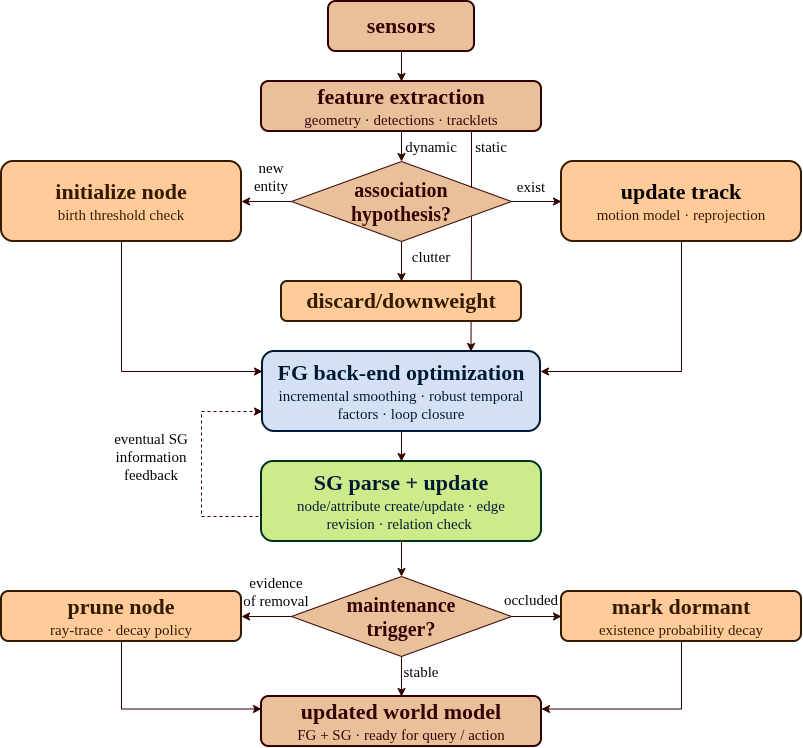
\includegraphics[width=\columnwidth]{Figures/figure_operational_pipeline.png}
    \caption{Per-frame operational pipeline of the hybrid world model.}
    \label{fig:FG_SG_world_model_construction_maintenance_workflow}
\end{figure}